\chapter{Experiments}

\section{Setup}

\begin{wrapfigure}{r}{0.4\textwidth}
  \begin{center}
    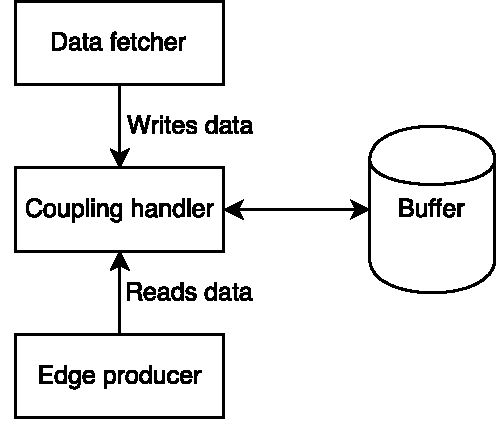
\includegraphics[width=0.38\textwidth]{Pipeline}
  \end{center}
  \caption{Parallel-compatible pipeline}
  \label{fig:pipeline}
\end{wrapfigure}

To do real-time experiments on a data-stream there are a few more tasks that needs to be performed in real-time. The three main tasks are: fetch data, produce graph edges, update DANF. To efficiently perform these tasks they are run in parallel. They are implemented as components of a pipeline as seen in figure \ref{fig:pipeline}. A component stores its results in a buffer which can be read by the component next in the pipeline. The writing component has write-only access and the reading component has read-only access. Note that Edge producer can be a writer to a DANF updater using another coupling handler. This makes it possible to create a theoretically infinite pipeline with very low coupling between components and allows every component to run in their own threads.

As all nodes and edges are handled as plain numbers, a mapping needs to be stored from node index to the data. Preferably the data should be stored in a database by a completely different machine. Otherwise the data management may take up too much processing power and memory. The only data that needs to be saved on the same machine is a mapping from node index to data index, which can be saved on disk.




\section{DANF vs HyperANF}

\section{Data retrieval}
What kind of information did we get from the data-sets?
